\section{Scene file format}
\label{sec:format}
Mitsuba uses a very simple and general XML-based format to represent scenes.
Since the framework's philosophy is to represent discrete blocks of functionality as plugins,
a scene file can essentially be interpreted as description that determines which
plugins should be instantiated and how they should interface with each other.
In the following, we'll look at a few examples to get a feeling for the scope of the
format.

A simple scene with a single mesh and the default lighting and camera setup might look
something like this:
\begin{xml}
<?xml version="1.0" encoding="utf-8"?>
<scene version=$\MtsVer$>
    <shape type="obj">
        <string name="filename" value="dragon.obj"/>
    </shape>
</scene>
\end{xml}
The scene version attribute denotes the release of Mitsuba that was used to
create the scene. This information allows Mitsuba to always correctly process the
file irregardless of any potential future changes in the scene description language.

This example already contains the most important things to know about format: you can have
\emph{objects} (such as the objects instantiated by the \code{scene} or \code{shape} tags),
which are allowed to be nested within each other. Each object optionally accepts \emph{properties}
(such as the \code{string} tag), which further characterize its behavior. All objects except
for the root object (the \code{scene}) cause the renderer to search and load a plugin from disk,
hence you must provide the plugin name using \code{type=".."} parameter.

The object tags also let the renderer know \emph{what kind} of object is to be instantiated: for instance,
any plugin loaded using the \code{shape} tag must conform to the \emph{Shape} interface, which is
certainly the case for the plugin named \code{obj} (it contains a WaveFront OBJ loader).
Similarly, you could write
\begin{xml}
<?xml version="1.0" encoding="utf-8"?>
<scene version=$\MtsVer$>
    <shape type="sphere">
        <float name="radius" value="10"/>
    </shape>
</scene>
\end{xml}
This loads a different plugin (\code{sphere}) which is still a \emph{Shape}, but instead represents
a sphere configured with a radius of 10 world-space units. Mitsuba ships with
a large number of plugins; please refer to the next chapter for a detailed
overview of them.

The most common scene setup is to declare an integrator, some geometry, a sensor (e.g. a camera), a film, a sampler
and one or more emitters. Here is a more complex example:
\begin{xml}
<?xml version="1.0" encoding="utf-8"?>

<scene version=$\MtsVer$>
    <integrator type="path">
        <!-- Path trace with a max. path length of 8 -->
        <integer name="maxDepth" value="8"/>
    </integrator>

    <!-- Instantiate a perspective camera with 45 degrees field of view -->
    <sensor type="perspective">
        <!-- Rotate the camera around the Y axis by 180 degrees -->
        <transform name="toWorld">
            <rotate y="1" angle="180"/>
        </transform>
        <float name="fov" value="45"/>

        <!-- Render with 32 samples per pixel using a basic
             independent sampling strategy -->
        <sampler type="independent">
            <integer name="sampleCount" value="32"/>
        </sampler>

        <!-- Generate an EXR image at HD resolution -->
        <film type="hdrfilm">
            <integer name="width" value="1920"/>
            <integer name="height" value="1080"/>
        </film>
    </sensor>

    <!-- Add a dragon mesh made of rough glass (stored as OBJ file) -->
    <shape type="obj">
        <string name="filename" value="dragon.obj"/>

        <bsdf type="roughdielectric">
            <!-- Tweak the roughness parameter of the material -->
            <float name="alpha" value="0.01"/>
        </bsdf>
    </shape>

    <!-- Add another mesh -- this time, stored using Mitsuba's own
         (compact) binary representation -->
    <shape type="serialized">
        <string name="filename" value="lightsource.serialized"/>
        <transform name="toWorld">
            <translate x="5" y="-3" z="1"/>
        </transform>

        <!-- This mesh is an area emitter -->
        <emitter type="area">
            <rgb name="radiance" value="100,400,100"/>
        </emitter>
    </shape>
</scene>
\end{xml}
This example introduces several new object types (\code{integrator, sensor, bsdf, sampler, film}, and \code{emitter})
and property types (\code{integer}, \code{transform}, and \code{rgb}).
As you can see in the example, objects are usually declared at the top level except if there is some
inherent relation that links them to another object. For instance, BSDFs are usually specific to a certain geometric object, so
they appear as a child object of a shape. Similarly, the sampler and film affect the way in which
rays are generated from the sensor and how it records the resulting radiance samples, hence they are nested inside it.

\subsection{Property types}
This section documents all of the ways in which properties can be supplied to objects. If you are more
interested in knowing which properties a certain plugin accepts, you should look at the next section instead.
\subsubsection{Numbers}
Integer and floating point values can be passed as follows:
\begin{xml}
<integer name="intProperty" value="1234"/>
<float name="floatProperty" value="1.234"/>
<float name="floatProperty2" value="-1.5e3"/>
\end{xml}
Note that you must adhere to the format expected by the object, i.e. you can't pass an integer property
to an object, which expects a floating-point value associated with that name.
\subsubsection{Strings}
Passing strings is straightforward:
\begin{xml}
<string name="stringProperty" value="This is a string"/>
\end{xml}
\subsubsection{Color spectra}
\label{sec:format-spectra}
Depending on the compilation flags of Mitsuba (see \secref{compiling-flags} for
details), the renderer internally either represents colors using discretized color spectra
(when \texttt{SPECTRUM\_SAMPLES} is set to a value other than 3), or it
uses a basic linear RGB representation\footnote{The official
releases all use linear RGB---to do spectral renderings, you will have
to compile Mitsuba yourself.}.
Irrespective of which internal representation is used, Mitsuba supports
several different ways of specifying color information, which is then
converted appropriately.

The preferred way of passing color spectra to the renderer is to explicitly
denote the  associated wavelengths of each value:
\begin{xml}
<spectrum name="spectrumProperty" value="400:0.56, 500:0.18, 600:0.58, 700:0.24"/>
\end{xml}
This is a mapping from wavelength in nanometers (before the colon)
to a reflectance or intensity value (after the colon).
Values in between are linearly interpolated from the two closest neighbors.
A useful shortcut to get a completely uniform spectrum, it is to provide
only a single value:
\begin{xml}
<spectrum name="spectrumProperty" value="0.56"/>
\end{xml}

Another (discouraged) option is to directly provide the spectrum in Mitsuba's
internal representation, avoiding the need for any kind of conversion.
However, this is problematic, since the associated scene will likely not work
anymore when Mitsuba is compiled with a different value of
\texttt{SPECTRUM\_SAMPLES}.
For completeness, the possibility is explained nonetheless. Assuming that
the 360-830$nm$ range is discretized into ten 47$nm$-sized blocks
(i.e. \texttt{SPECTRUM\_SAMPLES} is set to 10), their values can be specified
as follows:
\begin{xml}
<spectrum name="spectrumProperty" value=".2, .2, .8, .4, .6, .5, .1, .9, .4, .2"/>
\end{xml}

Another convenient way of providing color spectra is by specifying linear RGB
or sRGB values using floating-point triplets or hex values:
\begin{xml}
<rgb name="spectrumProperty" value="0.2, 0.8, 0.4"/>
<srgb name="spectrumProperty" value="0.4, 0.3, 0.2"/>
<srgb name="spectrumProperty" value="#f9aa34"/>
\end{xml}
When Mitsuba is compiled with the default settings, it internally uses
linear RGB to represent colors, so these values can directly be used.
However, when configured for doing spectral rendering, a suitable color
spectrum with the requested RGB reflectance must be found. This is a tricky
problem, since there is an infinite number of spectra with this property.

Mitsuba uses a method by Smits et al. \cite{Smits2005RGB} to find a
``plausible'' spectrum that is as smooth as possible. To do so, it uses
one of two methods depending on whether the spectrum contains a
unitless reflectance value, or a radiance-valued intensity.
\begin{xml}
<rgb name="spectrumProperty" intent="reflectance" value="0.2, 0.8, 0.4"/>
<rgb name="spectrumProperty" intent="illuminant" value="0.2, 0.8, 0.4"/>
\end{xml}
The \texttt{reflectance} intent is used by default, so remember to
set it to \texttt{illuminant} when defining the brightness of a
light source with the \texttt{<rgb>} tag.

When spectral power or reflectance distributions are obtained from measurements
(e.g. at 10$nm$ intervals), they are usually quite unwiedy and can clutter
the scene description. For this reason, there is yet another way to pass
a spectrum by loading it from an external file:
\begin{xml}
<spectrum name="spectrumProperty" filename="measuredSpectrum.spd"/>
\end{xml}
The file should contain a single measurement per line, with the corresponding
wavelength in nanometers and the measured value separated by a space. Comments
are allowed. Here is an example:
\begin{xml}
# This file contains a measured spectral power/reflectance distribution
406.13 0.703313
413.88 0.744563
422.03 0.791625
430.62 0.822125
435.09 0.834000
...
\end{xml}

\renderings{
    \fbox{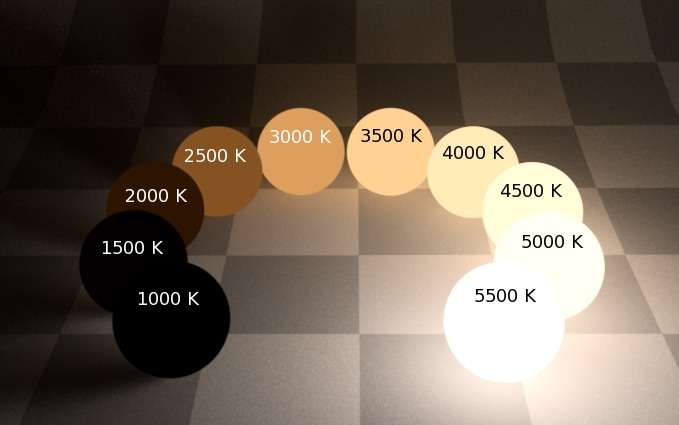
\includegraphics[width=10cm]{images/blackbody}}
    \hfill\,
    \caption{\label{fig:blackbody}A few simulated
    black body emitters over a range of temperature values}
}
\label{sec:blackbody}
Finally, it is also possible to specify the spectral distribution of a black body emitter (\figref{blackbody}),
where the temperature is given in Kelvin.
\begin{xml}
<blackbody name="spectrumProperty" temperature="5000K"/>
\end{xml}
Note that attaching a black body spectrum to the \texttt{intensity} property
of a emitter introduces physical units into the rendering process of
Mitsuba, which is ordinarily a unitless system\footnote{This means that the
units of pixel values in a rendering are completely dependent on the units of
the user input, including the unit of world-space distance and the units of
the light source emission profile.}.

Specifically, the black body spectrum has units of power ($W$) per
unit area ($m^{-2}$) per steradian ($sr^{-1}$) per unit wavelength ($nm^{-1}$).
If these units are inconsistent with your scene description, you may use the
optional \texttt{scale} attribute to adjust them, e.g.:
\begin{xml}
<!-- Scale black body radiance by a factor of 1/1000 -->
<blackbody name="spectrumProperty" temperature="5000K" scale="1e-3"/>
\end{xml}

\subsubsection{Vectors, Positions}
Points and vectors can be specified as follows:
\begin{xml}
<point name="pointProperty" x="3" y="4" z="5"/>
<vector name="vectorProperty" x="3" y="4" z="5"/>
\end{xml}
It is important that whatever you choose as world-space units (meters, inches, etc.) is
used consistently in all places.
\subsubsection{Transformations}
Transformations are the only kind of property that require more than a single tag. The idea is that, starting
with the identity, one can build up a transformation using a sequence of commands. For instance, a transformation that
does a translation followed by a rotation might be written like this:
\begin{xml}
<transform name="trafoProperty">
    <translate x="-1" y="3" z="4"/>
    <rotate y="1" angle="45"/>
</transform>
\end{xml}
Mathematically, each incremental transformation in the sequence is left-multiplied onto the current one. The following
choices are available:
\begin{itemize}
\item Translations, e.g.
\begin{xml}
<translate x="-1" y="3" z="4"/>
\end{xml}
\item Counter-clockwise rotations around a specified axis. The angle is given in degrees, e.g.
\begin{xml}
<rotate x="0.701" y="0.701" z="0" angle="180"/>
\end{xml}
\item Scaling operations. The coefficients may also be negative to obtain a flip, e.g.
\begin{xml}
<scale value="5"/>           <!-- uniform scale -->
<scale x="2" y="1" z="-1"/>  <!-- non-unform scale -->
\end{xml}
\item Explicit 4$\times$4 matrices, e.g
\begin{xml}
<matrix value="0 -0.53 0 -1.79 0.92 0 0 8.03 0 0 0.53 0 0 0 0 1"/>
\end{xml}
\item \code{lookat} transformations --- this is primarily useful for setting up cameras (and spot lights). The \code{origin} coordinates
specify the camera origin, \code{target} is the point that the camera will look at, and the
(optional) \code{up} parameter determines the ``upward'' direction in the final rendered image.
The \code{up} parameter is not needed for spot lights.
\begin{xml}
<lookat origin="10, 50, -800" target="0, 0, 0" up="0, 1, 0"/>
\end{xml}
\end{itemize}
Cordinates that are zero (for \code{translate} and \code{rotate}) or one (for \code{scale})
do not explicitly have to be specified.
\subsection{Animated transformations}
Most shapes, emitters, and sensors in Mitsuba can accept both normal transformations
and \emph{animated transformations} as parameters. The latter is useful to
render scenes involving motion blur (Figure~\ref{fig:animated-transform}). The syntax used to specify these
is slightly different:
\begin{xml}
<animation name="trafoProperty">
  <transform time="0">
     .. chained list of transformations as discussed above ..
  </transform>

  <transform time="1">
     .. chained list of transformations as discussed above ..
  </transform>

  .. additional transformations (optional) ..
</animation>
\end{xml}
\renderings{
 \fbox{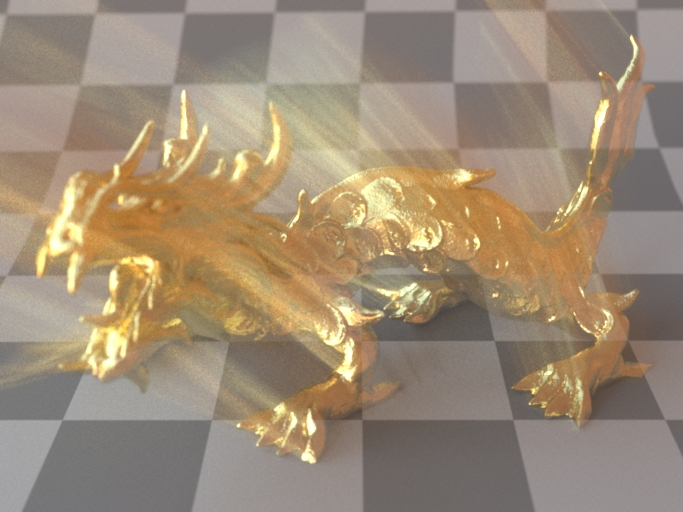
\includegraphics[width=.6\textwidth]{images/animated_transform}}\hfill\,
 \caption{\label{fig:animated-transform}Beware the dragon: a triangle mesh undergoing linear motion with several keyframes (object courtesy of XYZRGB)}
}

Mitsuba then decomposes each transformation into a scale, translation, and
rotation component and interpolates\footnote{Using linear interpolation
for the scale and translation component and spherical linear quaternion
interpolation for the rotation component.} these for intermediate
time values.
It is important to specify appropriate shutter open/close times
to the sensor so that the motion is visible.
\newpage
\subsection{References}
Quite often, you will find yourself using an object (such as a material) in many places. To avoid having
to declare it over and over again, which wastes memory, you can make use of references. Here is an example
of how this works:
\begin{xml}
<scene version=$\MtsVer$>
    <texture type="bitmap" id="myImage">
        <string name="filename" value="textures/myImage.jpg"/>
    </texture>

    <bsdf type="diffuse" id="myMaterial">
        <!-- Reference the texture named myImage and pass it
            to the BRDF as the reflectance parameter -->
        <ref name="reflectance" id="myImage"/>
    </bsdf>

    <shape type="obj">
        <string name="filename" value="meshes/myShape.obj"/>

        <!-- Reference the material named myMaterial -->
        <ref id="myMaterial"/>
    </shape>
</scene>
\end{xml}
By providing a unique \texttt{id} attribute in the
object declaration, the object is bound to that identifier
upon instantiation.
Referencing this identifier at a later point (using the \texttt{<ref id="..."/>} tag)
will add the instance to the parent object, with no further memory
allocation taking place. Note that some plugins expect their child objects
to be named\footnote{For instance, material plugins such as \pluginref{diffuse} require that
nested texture instances explicitly specify the parameter to which they want to bind (e.g. ``\texttt{reflectance}'').}.
For this reason, a name can also be associated with the reference.

Note that while this feature is meant to efficiently handle materials,
textures, and participating media that are referenced from multiple places,
it cannot be used to instantiate geometry---if this functionality is needed,
take a look at the \pluginref{instance} plugin.

\subsection{Including external files}
A scene can be split into multiple pieces for better readability.
to include an external file, please use the following command:
\begin{xml}
<include filename="nested-scene.xml"/>
\end{xml}
In this case, the file \code{nested-scene.xml} must be a proper scene file with a \code{<scene>} tag at the root.
This feature is sometimes very convenient in conjunction with the \code{-D key=value} flag of the \code{mitsuba} command line renderer (see the previous section for details).
This lets you include different parts of a scene configuration by changing the command line parameters (and without having to touch the XML file):
\begin{xml}
<include filename="nested-scene-$\texttt{\$}$version.xml"/>
\end{xml}
\subsection{Default parameter values}
As mentioned before, scenes may contain named parameters that are supplied via the command line:
\begin{xml}
<bsdf type="diffuse">
    <rgb name="reflectance" value="$\texttt{\$}$reflectance"/>
</bsdf>
\end{xml}
In this case, an error will occur when loading the scene without an explicit command line argument of the form
\code{-Dreflectance=}\mbox{$\langle$\emph{something}$\rangle$}. For convenience, it is possible to specify
a default parameter value that takes precedence when no command line arguments are given. The syntax for this is
\begin{xml}
<default name="reflectance" value="something"/>
\end{xml}
and must precede occurrences of the parameter in the XML file.

\subsection{Aliases}
Sometimes, it can be useful to associate an object (e.g. a scattering model)
with multiple identifiers. This can be accomplished using the \code{alias
as=..} keyword:
\begin{xml}
<bsdf type="diffuse" id="myMaterial1"/>
<alias id="myMaterial1" as="myMaterial2"/>
\end{xml}
After this statement, the diffuse scattering model will be bound to
\emph{both} identifiers ``\code{myMaterial1}'' and ``\code{myMaterial2}''.
